\clearpage 

\section{The impact of punctuated infectiousness profiles on uncontrolled epidemics}

\subsection{Punctuated individual infectiousness profiles generate later and more variably-timed epidemics.}

Early-outbreak stochasticity can impact when an epidemic becomes established, which in turn shifts the epidemic's full trajectory \citep{morris_computation_2024}. Simulations demonstrate that narrower $a_i(\tau)$ (\ie, $\psi \rightarrow 0$) cause this time shift's expected value to move later and its variance to increase. For 5,000 simulations across each of the three benchmark pathogens and for $\psi \in \{0, 0.5, 1\}$, we measured the time to reach 5\% cumulative prevalence (\ie, 500 total infections), which we took as a marker of epidemic establishment. For influenza, the mean [5\% quantile, 95\% quantile] time to reach 500 cases was 24.2 days [17.8, 33.8] for $\psi = 1$ and 24.5 [17.2, 34.9] for $\psi = 0$; for omicron, 18.1 days [14.8, 22.9] for $\psi = 1$ and 20.3 days [13.4, 30.4] for $\psi = 0$; and for measles, 31.3 days [28.6, 34.6] for $\psi = 1$ and 32.5 days [26.4, 39.5] for $\psi = 0$. These results indicate that the $\psi$-effect was amplified for pathogens with higher $R_0$ (omicron, measles). This translated into meaningful differences in epidemic timing, particularly for SARS-CoV-2 omicron and measles: on day 20, 82\% of simulated SARS-CoV-2 omicron outbreaks with $\psi = 1$ had reached 500 cases, while only 55\% of outbreaks with $\psi = 0$ had reached the same threshold. Similarly, by day 33, 84\% of simulated measles outbreaks with $\psi = 1$ had reached 500 cases, while only 58\% of outbreaks with $\psi = 0$ had reached the same threshold ({\bf Figure \ref{fig:survival}}). 

% by day , 89\% of simulated SARS-CoV-2 omicron outbreaks with $\psi = 1$ had reached 500 cases, while only 62\% of outbreaks with $\psi = 0$ had reached the same threshold. Similarly, by day 35, 96\% of simulated measles outbreaks with $\psi = 1$ had reached 500 cases, while only 76\% of outbreaks with $\psi = 0$ had reached the same threshold ({\bf Figure \ref{fig:survival}}). 

Analytic results rooted in branching theory confirm that these trends hold more generally. Let $Z(t)$ be the cumulative number of individuals infected at time $t$; then, following \citet{morris_computation_2024}, we can define a rescaled branching process 
\begin{equation}
	W(t) = e^{-r t} Z(t)
\end{equation}
with initial condition $W(0)$ and growth rate $r$ that describes the epidemic's exponential growth phase. The process $W(t)$ converges almost surely to a random variable $W$, which can be loosely interpreted as random initial condition on the branching process that captures the effect of early-outbreak stochasticity. With a change of variables, this random initial condition can be expressed as a random time shift $\varsigma$, where 
\begin{equation}
	\varsigma = \frac{\log W - \log E[W]}{r}
\end{equation}
and the branching process can be expressed as 
\begin{equation}
	Z(t) \approx e^{r(t + \varsigma)}
\end{equation}
For notational simplicity, we assume that epidemics are always seeded with a single infectious case; thus, $E[W] = Z_0 = 1$ and $\varsigma = \log W / r$. 

Under the Gamma time-shift model for $a_i(\tau)$, we can derive the variance of the random initial condition ({\bf Supplementary Methods}): 
\begin{equation}
	\text{Var}[W] = \frac{
		\Bigl(\frac{1 + z}{1 + 2z}\Bigr)^\alpha + \Bigl(\frac{(1 + z)^2}{1 + 2z}\Bigr)^{(1-\psi) \alpha} - 1
	}{
		1 - \Bigl(\frac{1 + z}{1 + 2z}\Bigr)^\alpha
	} := 
	\frac{\sigma_1^\alpha + \sigma_2^{(1-\psi)\alpha} - 1}{1 - \sigma_1^\alpha}
	\label{eq:var_W}
\end{equation}
where $z = R_0^{1/\alpha} - 1$ and $\sigma_c = ((1+z)^c) / (1 + 2z)$. Thus, $\text{Var}[W]$ depends on $R_0$, $\alpha$ (\ie, the shape/skewness of $A(\tau)$), and $\psi$. The punctuation parameter $\psi$ enters Eq.~\ref{eq:var_W} only once, in the exponent of $\sigma_2$. Since $\sigma_2 > 1$ when $R_0 > 1$, $\text{Var}[W]$ and $\psi$ are monotonically related, where narrower individual infectiousness profiles ($\psi \rightarrow 0$) maximize the variance and broader profiles ($\psi \rightarrow 1$) minimize it. Furthermore, $\sigma_2$ is monotonically increasing in $R_0$ ({\bf Supplementary Methods}), so larger $R_0$ amplifies the dependence of $\text{Var}[W]$ on $\psi$. If we further assume, following \citet{morris_computation_2024}, that the distribution of $W$ is well approximated by a $\text{Gamma}(k, \lambda)$ distribution with first two moments matched to those of $W$, we can derive closed-form expressions for $E[\varsigma]$ and $\text{Var}[\varsigma]$ ({\bf Supplementary Methods}). These confirm that higher $\text{Var}[W]$ --- and thus narrower infectiousness profiles --- lead to more negative $E[\varsigma]$ (\ie, cause the expected time shift to fall later) and higher $\text{Var}[\varsigma]$. 

These analytic results also apply more generally than the Gamma time-shift model for $a_i(\tau)$. For any probability densities $f_l$ and $f_\epsilon$ that define an individual latent period and infectiousness kernel, such that $f_l (\tau)\circ f_\epsilon(\tau) = g(\tau)$, it can be shown that decreasing the variance of $f_\epsilon(\tau)$ increases the variance of $W$, with the effect size modulated by $R_0$ ({\bf Supplementary Methods}). If we assume the distribution of $W$ is well-approximated by a Gamma distribution, the effects of $f_\epsilon$'s variance on $E[\varsigma]$ and $\text{Var}[\varsigma]$ follow as before. 

Intuitively, this $\psi$-dependent difference in the time shift's distribution arises from an order statistics phenomenon combined with exponential growth. For smooth infectiousness profiles ($\psi = 1$), the timing of each secondary infection is drawn independently from $g(\tau)$. As $R_0$ grows, the earliest of these infections happens increasingly sooner, giving the epidemic an early start. In terms of epidemic growth, these early infections matter exponentially more than the later ones. For punctuated profiles ($\psi = 0$), by contrast, all secondary infections cluster around a single random time drawn from $g(\tau)$. While this avoids the smooth profile's late infections, it also misses out on the advantage provided by the early ones --- and that missed advantage turns out to matter more, in terms of the expected time shift. [Something about skewness here is important for the expected time shift.] Similarly, the tight clustering of secondary infections for punctuated infectiousness profiles amplifies the impact of draws from $g(\tau)$ that lie in the tail, increasing the variance of the epidemic's effective start time. 

% The intuition behind these timing effects rests on a temporal diversification argument. Consider an index case who produces $R_0$ secondary infections on average. Under a smooth infectiousness profile ($\psi = 1$), each secondary infection occurs at an independently drawn time from the generation interval distribution $A(\tau)$. As $R_0$ grows, the \emph{earliest} of these independent draws falls increasingly close to the left edge of $A(\tau)$ --- an order-statistic effect --- giving the epidemic a reliably early start. Under a punctuated profile ($\psi \approx 0$), by contrast, all secondary infections cluster around a single random time drawn from $A(\tau)$. There is no diversification: the ``earliest'' transmission is simply the single draw itself, regardless of $R_0$. When this draw falls in the right tail of $A(\tau)$, the entire packet of $\sim R_0$ infections arrives late, delaying the epidemic; when it falls in the left tail, they all arrive early, accelerating it. This all-or-nothing timing inflates both the variance and the mean delay of epidemic establishment.

% The roles of $R_0$ and the shape of $A(\tau)$ follow naturally. Higher $R_0$ amplifies the diversification advantage of smooth profiles --- more independent draws make the order-statistic minimum more extreme --- while offering no such benefit to punctuated profiles, since a single shared draw is a single shared draw regardless of how many infections it carries. More right-skewed generation interval distributions (smaller shape parameter $\alpha$, for fixed mean) extend the right tail of $A(\tau)$, increasing the chance that a punctuated individual's single draw falls far from the mode and creating more extreme timing outliers. Both effects are visible in the simulations: the sensitivity of epidemic timing to $\psi$ is greatest for measles (highest $R_0$) and for SARS-CoV-2 omicron (most right-skewed generation interval).

% Crucially, this diversification mechanism does not depend on the specific time-shifted Gamma model used here. The key structural feature is that punctuated profiles reduce the number of \emph{independent} timing draws contributing to early transmission: when secondary infections share a common latent period or burst time, they lose the variance-reducing benefit of temporal independence. Any model in which narrower infectiousness profiles increase the correlation among an individual's secondary infection times --- whether through a shared latent period, a concentrated burst of infectiousness, or a narrow window of high contact --- will produce the same qualitative pattern. The formal requirement is mild: the generation interval distribution must be non-degenerate and unimodal, so that temporal diversification has scope to operate and a single draw is meaningfully riskier than several independent draws. Under these conditions, the analytic results derived below for the time-shifted Gamma model should be understood as capturing a robust, general phenomenon rather than a model-specific artifact.

\begin{figure}[ht] 
\centering
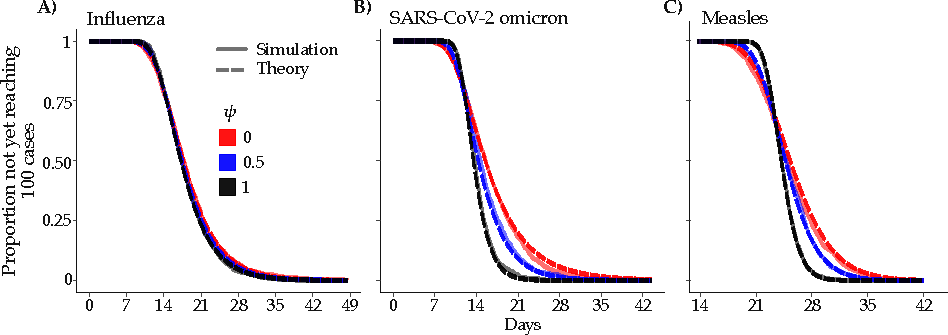
\includegraphics[width=\textwidth]{survival.pdf}
\caption{{\bf \boldmath Proportion of epidemics not yet reaching 100 infections for three pathogens.}  }
\label{fig:survival}
\end{figure}

% ////////////////////////////////////////////////////////////////////////////////////////////

\subsection{Narrow individual infectiousness profiles yield greater uncertainty in epidemic growth rate estimates}

Punctuated individual infectiousness profiles also make empirical estimates of the early-epidemic exponential growth rate $r$ more uncertain ({\bf Figure XX}). 

% ////////////////////////////////////////////////////////////////////////////////////////////

\subsection{Narrow biological infectiousness profiles interact with periodic contact patterns to generate overdispersion in secondary infections}

When each person has the same inherent infectiousness ($\nu_i \equiv R_0$) and contacts are uniform across individuals and over time ($c_i(t) \equiv \bar{c} = 1$), the timing of a person's secondary infections ($\xi_i(\tau)$) has no effect on the secondary infection distribution: every person produces a $\text{Poisson}(R_0)$-distributed number of infections. However, if contacts vary over time and/or across individuals, overdispersion may emerge as the interaction between $\xi_i$ and $c_i(t)$ produce variation in the realized individual reproduction number, $\nu_i^{\text{re}}$. 

The periodic contact model introduces temporal, but not interpersonal, variation in contacts. 

Similar results hold under the Gamma contact model, which introduces both temporal and interpersonal variation in contacts, but holds the population-average contact rate at $C(t) = 1$. 

%
\begin{equation}
	k = \frac{2}{A^2}\left(1 + \frac{\omega^2}{\beta^2}\right)^{\psi \alpha}
	\label{eq:k_periodic_main}
\end{equation}
%
where $A$ is the amplitude of the contact oscillation and $\omega$ is its angular frequency. Here, the prefactor $2/A^2$ sets the overall overdispersion scale, and the bracketed factor quantifies the failure of the biological profile's temporal window to average out the contact oscillation, with $(1 + \omega^2/\beta^2)^{-\psi\alpha}$ being exactly the squared characteristic function of the Gamma$(\psi\alpha, \beta)$ density at the contact frequency $\omega$. Since this factor is strictly increasing in $\psi$ for any $\omega > 0$, narrower biological profiles always produce more overdispersion in the presence of periodic contact variation. The effect disappears in the spike limit only if $\omega \rightarrow 0$ or $A \rightarrow 0$ (no temporal contact variation), and grows arbitrarily large in the smooth limit if $\omega/\beta$ is large (contact oscillations much faster than the profile window, so the profile averages them out). Simulations extend this result to heavier-tailed, non-periodic contact heterogeneity, for which the same mechanism holds qualitatively ({\bf Figure XX}).

% Even in large, well-mixed populations, stochasticity can durably impact the trajectory of an epidemic. One way this stochasticity enters is via a random time shift, where epidemics take a variable amount of time to reach the exponential growth phase \citep{morris_computation_2024}, leading to variation in the timing of the entire epidemic trajectory. Here, we address the question of how this time shift distribution depends on the shape of the individual infectiousness profile, holding all else equal. 

% Simulations confirm that narrower infectiousness profiles ($\psi \rightarrow 0$) yield more variable and later-shifted epidemic timings ({\bf Figure XX}, {\bf Supplementary Table Sxx}). Across 10,000 simulated epidemics in a population of size 1000 using SARS-CoV-2 omicron-like parameters, the median time to reach 100 infections was XX days for $\psi = 0$ (IQR: [XX, XX]) vs. XX days for $\psi = 1$ (IQR: [XX, XX]). The impact of $\psi$ on epidemic timing was lessened with lower $R_0$ (influenza-like parameters, median time to 100 infections: XX days for $\psi=0$ [IQR: XX, XX] vs. XX days for $\psi=1$ [IQR: XX, XX]) and increased with higher $R_0$ (measles-like parameters, median time to 100 infections: XX days for $\psi=0$ [IQR: XX, XX] vs. XX days for $\psi=1$ [IQR: XX, XX]). From another perspective: by day XX of the simulated epidemic under measles-like parameters, XX\% of the outbreaks with $\psi = 1$ had reached 100 infections, while only XX\% of the outbreaks with $\psi=0$ had reached 100 infections ({\bf Figure XX}). 

% These observations are confirmed by the underlying theory. The cumulative incidence over time, $Z(t)$, during the early exponential growth phase of an epidemic can be approximated as a deterministic exponential growth function with a random initial condition scaling factor $W$: 

% \begin{equation}
% 	Z(t) \approx W \cdot ce^{rt}
% \end{equation}

% with exponential growh rate $r$, and where $c$ is the mean-field initial condition (when $W = 1$). 

% With a change of variables, the cumulative incidence can be expressed as the same deterministic growht function with a random time shift $\varsigma$: 

% \begin{equation}
% 	Z(t) \approx c e^{r(t+\varsigma)}
% \end{equation}

% where 

% \begin{equation}
% 	\varsigma = \frac{\log W - \log E[W]}{r}
% \end{equation}

% Here, $E[W]$ is the initial condition and $r$ is the exponential growth rate, so $\varsigma \propto \log[W]$. 

% First, we consider the variance of the time shift, $Var[\varsigma]$. For ease of notation, we focus on $Var[W]$, noting that $Var[\varsigma]$ is monotonically related to $Var[W]$. It can be shown that {\bf Supplementary Text}

% \[ 
% Var[W] = m_2 + R_0^2 \rho^{2 \psi \alpha} [\rho_2^{(1-\psi)\alpha} - \rho^{2(1-\psi)\alpha}]
% \]

% which is maximized when $\psi = 0$ (the infectiousness profile is narrow) and becomes 0 when $\psi = 1$ (the infectiousness profile is maximally broad). (Can we say something about how this suggests that the variance of the time shift scales roughly linearly with $\psi$?)

% Next, we consider the typical time shift, which we obtain by studying the mode of the distribution of $W$. 

% Let $I_b(t)$ be the (stochastic) number of infections at time $t$ for a single epidemic realization, where the subscript ``b'' marks that it is a branching process. Let $I_d(t)$ be its mean-field deterministic counterpart. Then, we can approximate $I_b(t)$ as $I_d(t+\varsigma)$, {\it i.e.,} the branching process is approximately equal to the deterministic process with a random time shift. 

% The time shift is 

% \[ \varsigma = \frac{\log W - \log E[W]}{r}\]

% where $r$ is the epidemic's exponential growth rate and $W = \lim_{t \rightarrow \infty} W(t)$ is the limiting value of the rescaled branching process $W(t) = e^{-r t I_b(t)}$. The process $W(t)$ is well studied, and knowing its distribution fully determines the distribution of the time shift $\varsigma$. 

% The expectation of $W$ is equal to the initial condition ($E[W] = I_0$). For simplicity, we will assume $I_0 = 1$ throughout this section, though the findings can be easily extended to general initial conditions. Here, we assess the impact of the individual infectiousness profile's breadth, $\phi$, on (a) the variance of $W$ and (b) the mode of a Gamma approximation to W obtained via moment matching. 

% It can be shown that 

% \[ \text{Var}(W) = \frac{c^\alpha + \sigma^{(1-\psi) \alpha} - 1}{1 - c^\alpha} \]

% \noindent where $c$ depends on $R_0$ and $\alpha$ but not $\psi$. Thus, broad profiles ($\psi \rightarrow 1$) minimize $\text{Var}(W)$ and narrow profiles ($\psi \rightarrow 0$) maximize it. 

% We can approximate the distribution of $W$ using moment matching to a generalized Gamma distribution. With the Gamma-shaped individual infectiousness profiles, the moments have closed-form expressions. Using two-moment matching to a Gamma distribution, we find that 

% \[ \text{mode}_\varsigma = \frac{1}{r} \log(1 - \text{CV}^2_\text{cond})] \]

% Here, (description). Again, we see that the mode shifts later as $\psi \rightarrow 0$. 

% The theory aligns well with the simulations. Using generalized gamma distributions fit using moment matching to the first five moments of $W$, we get similar survival curves for the time to 100 infected ({\bf Figure XX}). 

% \subsection{Narrower individual infectiousness profiles yield greater uncertainty in epidemic growth rate estimates.}

% Based on simulations. 

% \subsection{Narrower biological infectiousness profiles interact with periodic contact patterns to generate overdispersion in secondary infections.}

% Closed-form solution: 

% \[ k = \frac{2}{\bar{c}^2}{A^2} \Bigl(1 + \frac{\omega^2}{r^2}\Bigr)^{\psi \alpha} = \frac{2}{\bar{c}^2}{A^2} \Bigl(1 + (\frac{z^*_{per}}{z_{per}})^2\Bigr)^{\psi \alpha} \]



% \begin{figure}[ht]
% \centering
% 
\includegraphics[width=.5\textwidth]{figures/stock.png}
% \caption{{\bf Impact of the individual infectiousness profile on epidemic timing.} Survival curves for time-to-100. growth rate estimate box-and-whiskers. Overdispersion/k vs psi heatmap.} 
% \label{fig:uncontrolled}
% \end{figure}


% Stepwise, smooth, and spike all yield the same mean dynamics
% Stepwise has higher extinction probability, explained by overdispersion
% Spike has later and more variable establishment properties, including time-to-n-infected and peak, and exponential growth rate is more variable. We can show this through simulations and through analytic approaches, following Morris' time shift ideas \citep{morris2024}

% With constant contacts, kappa doesn't affect extinction or overdispersion -- only growth timing

% but introduce time-varying contacts and suddenly kappa controls overdispersion

% Spike emphasizes variation in contacts, leading to overdispersion.
